\chapter{跑步} \label{chap:chap3}

如果你能用六十秒的长跑来填补这无情的一分钟……
\begin{flushright}
	——拉迪亚德$\cdot$吉卜林
\end{flushright}


\begin{figure}[!htb]
	\centering
	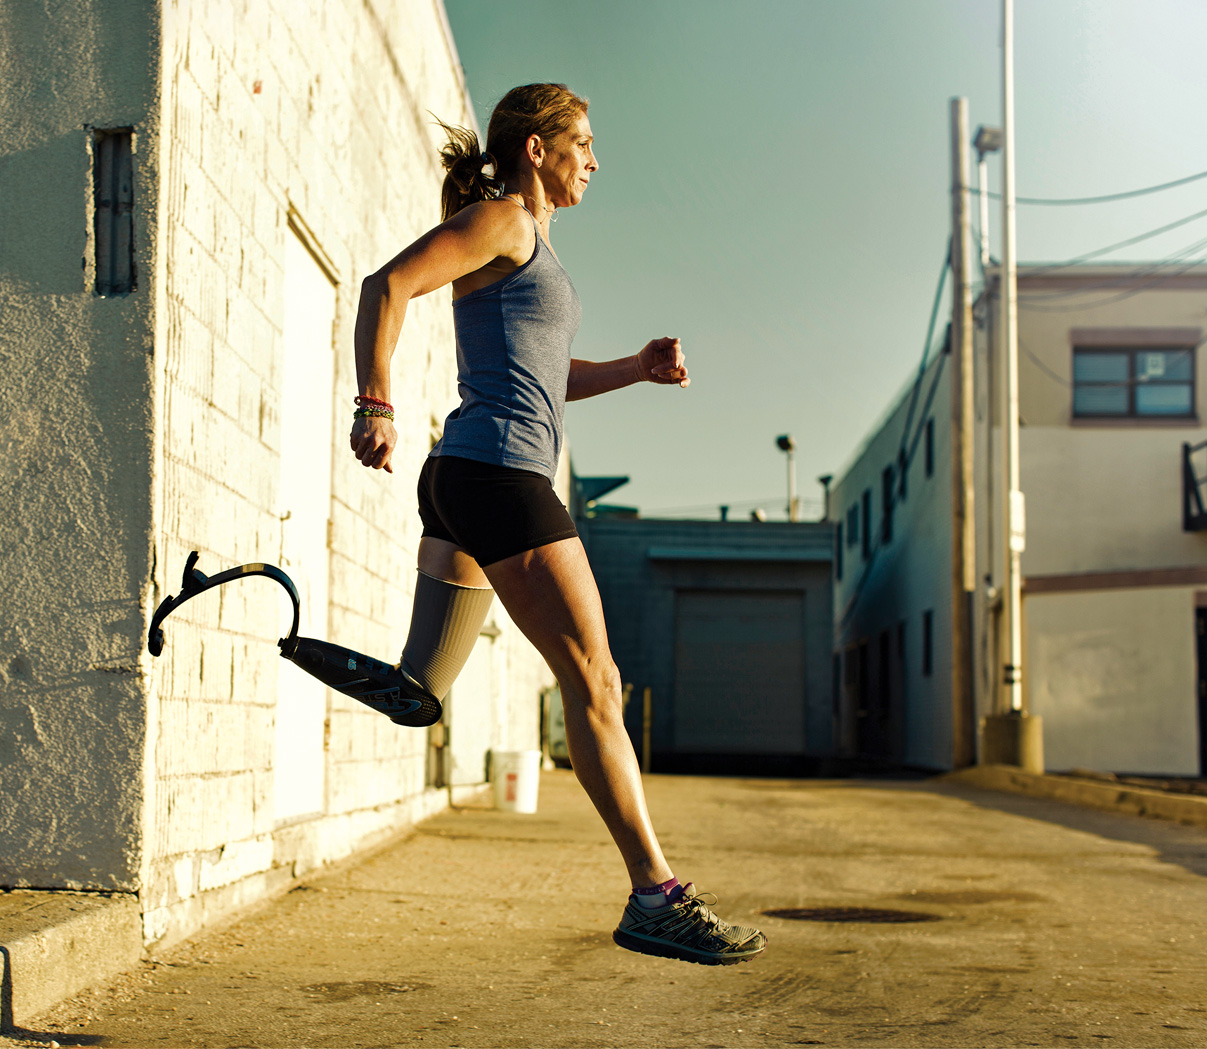
\includegraphics[width=1.0\linewidth]{chap3/3_0}
	% 加星号(*)表示不加编号
	\caption*{ \label{fig:3_0}}
\end{figure}

看过《侏罗纪公园》的人可能都记得那个标志性的场景:
一辆吉普车试图超越一只追赶的霸王龙。
有趣的是,这个场景与电影上映时(1993年)古生物学家的普遍看法相符。
当时人们认为霸王龙的奔跑速度可以达到 40 公里/小时,一些科学家甚至认为它的速度甚至可能更快。
以这样的速度,它在土路上完全可以超过一辆吉普车。


然而,自 2002 年约翰$\cdot$哈钦森(John Hutchinson)开创性论文以来,近期的生物力学研究表明,霸王龙可能根本无法奔跑。
即使它能跑,也可能无法达到 40 公里/小时的速度。
哈钦森通过模拟霸王龙,证明要达到这样的速度,其 86\% 的体重必须由腿部肌肉构成,留给其庞大的尾巴、头部和躯干的空间非常有限。
为了产生足够大的地面反作用力,它需要将如此大的质量分配给腿部肌肉,而这种反作用力在奔跑时通常超过体重的两倍。


对恐龙、大象和袋鼠等动物的研究有助于我们理清对人类跑步的理解:
是什么驱动着从步行到跑步的转变,又是什么限制了跑步速度。
地面反作用力的测量揭示了为什么跑步时比步行时更容易受伤,以及如何设计跑道来降低受伤率并提高速度。


在本章中,我们将使用简单的力学模型来探讨这些问题。
这些模型包含弹簧,用于表示肌肉和肌腱的弹性特性,并揭示弹性能量的储存和释放如何提高跑步效率。
首先,我们定义跑步步态周期,并研究其中涉及的力和弹性机制。
然后,我们将探索一些原理,帮助你设计跑道、跑鞋和假肢,从而实现快速高效的跑步。
我们还会研究从步行过渡到跑步时步态和能量消耗的变化。


\section{跑步步态周期}

跑步步态周期由单腿支撑和腾空交替的阶段组成(图~\ref{fig:3_1})。
与步行类似,一个跑步步态周期由同一条腿连续 2 次触地事件定义,其中对侧腿的触地发生在半程。
每条腿都有一个\textit{支撑期}(脚与地面接触)和一个\textit{摆动期}(脚离地)。
支撑期始于脚触地,结束于脚趾离地,在人类跑步过程中约占步态周期的 30\% 到 45\%,但在高速冲刺过程中可能只占 25\% 或更少。
回想一下,步行时支撑期的持续时间会随着步行速度的增加而缩短。
因此,随着步行速度的增加,双腿支撑的持续时间会缩短。
如果进一步提高速度,每条腿对应的支撑期最终将持续不到步态周期的一半,从而进入腾空期。


\begin{figure}[!htb]
	\centering
	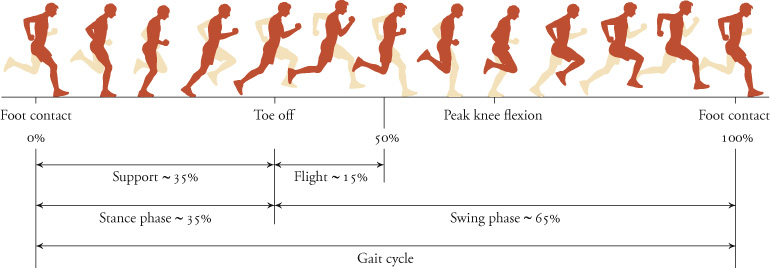
\includegraphics[width=1.0\linewidth]{chap3/3_1}
	\caption{跑步步态周期及其组成事件(例如,脚部触地)和阶段(例如,支撑)。
		站立和摆动的时间百分比会随着跑步速度和风格而变化。 \label{fig:3_1}}
\end{figure}

腾空阶段的存在是我们区分行走和跑步的一个方式。
事实上,人们很容易相信它是跑步的特征,不仅对人类如此,对其他动物也是如此。
然而,我们很快就会看到,当我们从行走步态转换为跑步步态时,会发生另一种质的变化,从生物力学的角度来看,这一点更为重要。


用于量化跑步步态周期的指标与用于步行的指标类似。
步长是两个连续足迹之间沿行进线的距离。
连续两步所走的距离,或一个步态周期所走过的距离,称为步长。
足部接触事件发生的速率(相当于步长持续时间的倒数)称为步频;
迈步的速率称为步频。
跑步速度可以用步长与步频的乘积来计算,
或者,也可以用步长与步频的乘积来计算:

\begin{equation}
	\text{速度(米/秒)} = \text{步长(米/步)} \times \text{节律(步/秒)} \label{eq:3_1}
\end{equation}

中等跑步速度为 4 米/秒。
在此速度下,支撑期约占步态周期的 35\% 至 40\%,典型的步频为 180 步/分钟,典型的步长约为 1.3 至 1.4 米:

\begin{equation}
	\text{步长} = \frac{4.0 \text{米}}{1 \text{秒}}
				 \times \frac{60 \text{秒}}{1 \text{分钟}}
				 \times \frac{1 \text{分钟}}{180 \text{步}}
				 = 1.33 \text{米/秒}
				 \label{eq:3_2}
\end{equation}

当然,这些数量会随着腿长、跑步风格、鞋类和其他因素而变化。












